\documentclass[10pt]{beamer}

\usepackage{ucs}
\usepackage[utf8x]{inputenc}
\usepackage{beamerthemeshadow}
\usepackage{amsmath}
\usepackage[british]{babel}
\usepackage{fontenc}
\usepackage{graphicx}
\usepackage{tikz}
\usetikzlibrary{arrows,positioning}
\usetikzlibrary{shapes,snakes}

\usepackage{xcolor}
\definecolor{olive}{rgb}{0.3, 0.4, .1}
\definecolor{gold}{rgb}{1.,0.,0.}

\title{An Introduction to Python}
\author{William Vigor and Clyde Fare}
\date{}
\newcommand{\bra}[1] { \langle #1 | }
\newcommand{\ket}[1] { | #1 \rangle }
\newcommand{\bket}[1] { \langle #1  \rangle }
\newcommand{\brket}[2] { \langle #1 | #2 \rangle }
\newcommand{\braket}[3] { \langle #1 | #2 | #3 \rangle }
\newcommand{\ketbra}[1] {\ket{#1}\bra{#1}}
\begin{document}

\maketitle
\titlegraphic{
\includegraphics[width=0.5\textwidth]{Imperial_2_Pantones.pdf}
}
\frame{
        \frametitle{Philosophy of the Course}
\begin{itemize}
\item Hands on: only this short introductory talk. No one wants to listen to lectures about how to program.
\item 3 Workshops:
\end{itemize}
\begin{enumerate}
\item Introducing the basics of python.
\item Using Python for science and data analysis.
\item Advanced Python.
\end{enumerate}


}
\part{Introduction: What is Programming ?}
\frame{\partpage}


\frame{
        \frametitle{What is programming ?}
\begin{itemize}
\item A Computer Program :
\end{itemize}
``A sequence of instructions that a computer can interpret and execute "
\begin{itemize}
\item In scientific programming these instructions are used to either analyse experimental data or for computational simulation. 
\end{itemize}

\begin{itemize}
\item Scientific simulations run on many of the fastest computers in the world. (10,000's of CPUs)
\end{itemize}


\begin{exampleblock}{}
\begin{figure}
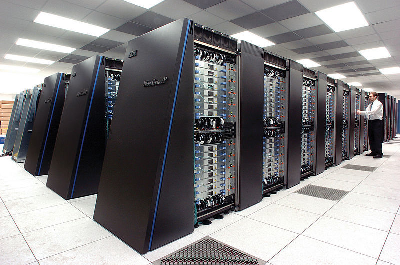
\includegraphics[width=0.5\textwidth]{supercomputer.pdf}
\end{figure}
\end{exampleblock}


}


\frame{
        \frametitle{Why Programming is Hard}
\begin{itemize}
\item Computers are dumb - they can only follow the simplest of instructions.
\item Computers are obedient but have no empathy.
\end{itemize}
\vspace*{1\baselineskip}
`` Computers are good at following instructions, but not at reading your mind. " - Donald Knuth \\
\vspace*{1\baselineskip}
``As soon as we started programming, we found to our surprise that it wasn’t as easy to get programs right as we had thought. Debugging had to be discovered. I can remember the exact instant when I realised that a large part of my life from then on was going to be spent in finding mistakes in my own programs."
- Maurice Wilkes \\
}

\frame{
        \frametitle{Why Learn to program}
\begin{itemize}
\item Experimental equipment is now commonly computerised.
\item A powerful tool to analyse experimental data more efficiently.
\item Write computer simulations to complement experimental data.
\item A useful transferable skill.
\end{itemize}

}

\frame{
        \frametitle{Why Learn to program}
\begin{itemize}
\item Make science reproducible:
\item A program run once with the same inputs should produce the same results if run again.
\end{itemize}
}


\part{Why Python ?}
\frame{\partpage}

\frame{
	\frametitle{Python Versus other Languages}
\begin{itemize}
\item Easy to learn but powerful.
\item Python's syntax is designed to be readable.
\end{itemize}

\begin{exampleblock}{}
\begin{columns}
\begin{column}{0.5\textwidth}
\centering
\textcolor{gold}{for} i \textcolor{gold}{in} $[$0, 1, 2, 3, 4, 5$]$:\\ 
\textcolor{olive}{print}(i)\\
\end{column}

\begin{column}{0.5\textwidth}
\textcolor{olive}{\#include $\langle$ stdio.h $\rangle$}\\
\textcolor{gold}{int} main(void)\\
\{\\
\hspace*{0.33cm}\textcolor{gold}{for} (\textcolor{gold}{int} i=0; i$<$6; i$++$)\\
\hspace*{0.33cm}\{\\
\hspace*{0.33cm}\hspace*{0.33cm} printf(``\%i \textbackslash n", i);\\
\hspace*{0.33cm}\}\\
\hspace*{0.33cm}\textcolor{gold}{return}(0);\\
\}
\end{column}

\end{columns}

\end{exampleblock}

\begin{itemize}
\item No need to worry about low level machine details (e.g. memory allocation in C).
\item Easy to run - no need for compilation.
\end{itemize}

}
\frame{
	\frametitle{Python Versus other Languages}
\begin{itemize}
\item Batteries included: No need to reinvent the wheel:
\item Many open source scientific and other libraries available.
\item e.g. Matplotlib for plotting
\end{itemize}
\begin{exampleblock}{}
\begin{figure}
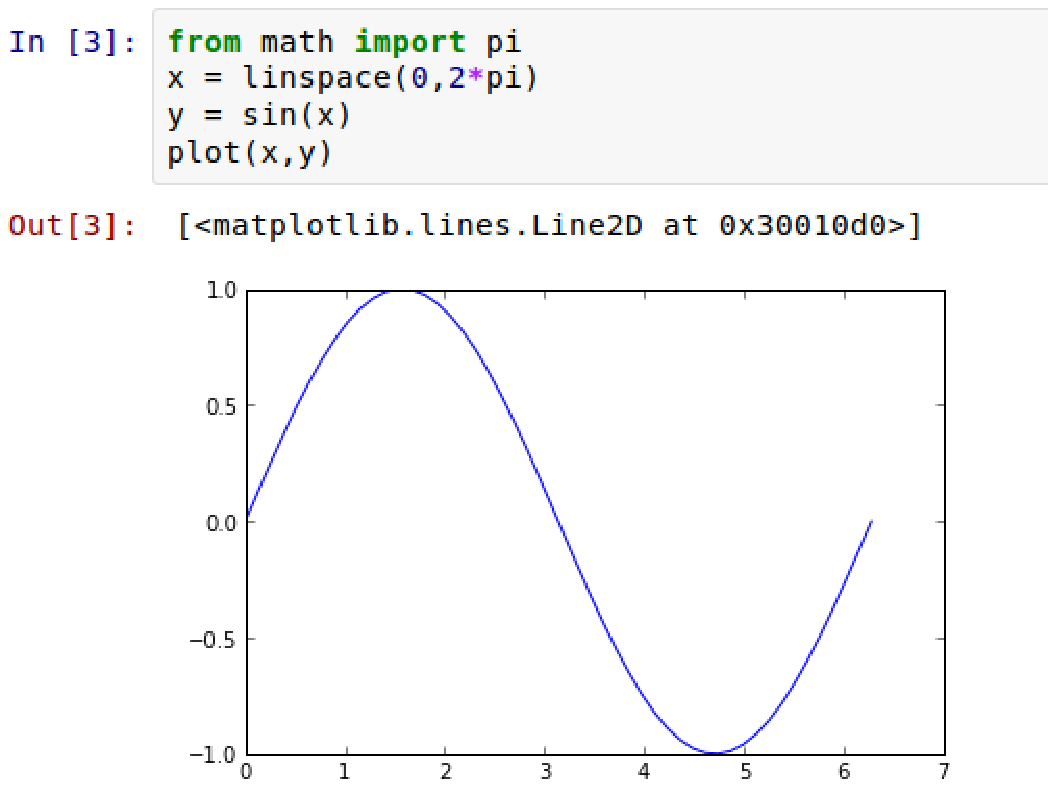
\includegraphics[width=0.5\textwidth]{sinx.pdf}
\end{figure}
\end{exampleblock}
}




\frame{
	\frametitle{Python is Open source}

\begin{itemize}
\item No need to buy a license, can use it at home even after you leave Imperial.
\item Compatible across multiple platforms Linux, Mac, Windows.
\item The Python community is very active a large group of people are continually developing new features.
\item If a feature is not present then you can add it in yourself might be useful for others.
\item You can look at the code to check it is doing what you think it's doing.
\end{itemize}
}


\part{How to can we run Python}
\frame{\partpage}
\frame{
	\frametitle{From the Command Line}
\begin{itemize}
\item Put python code into .py file using a text editor.
\item Run on the command line: python test.py 
\end{itemize}

\begin{exampleblock}{}
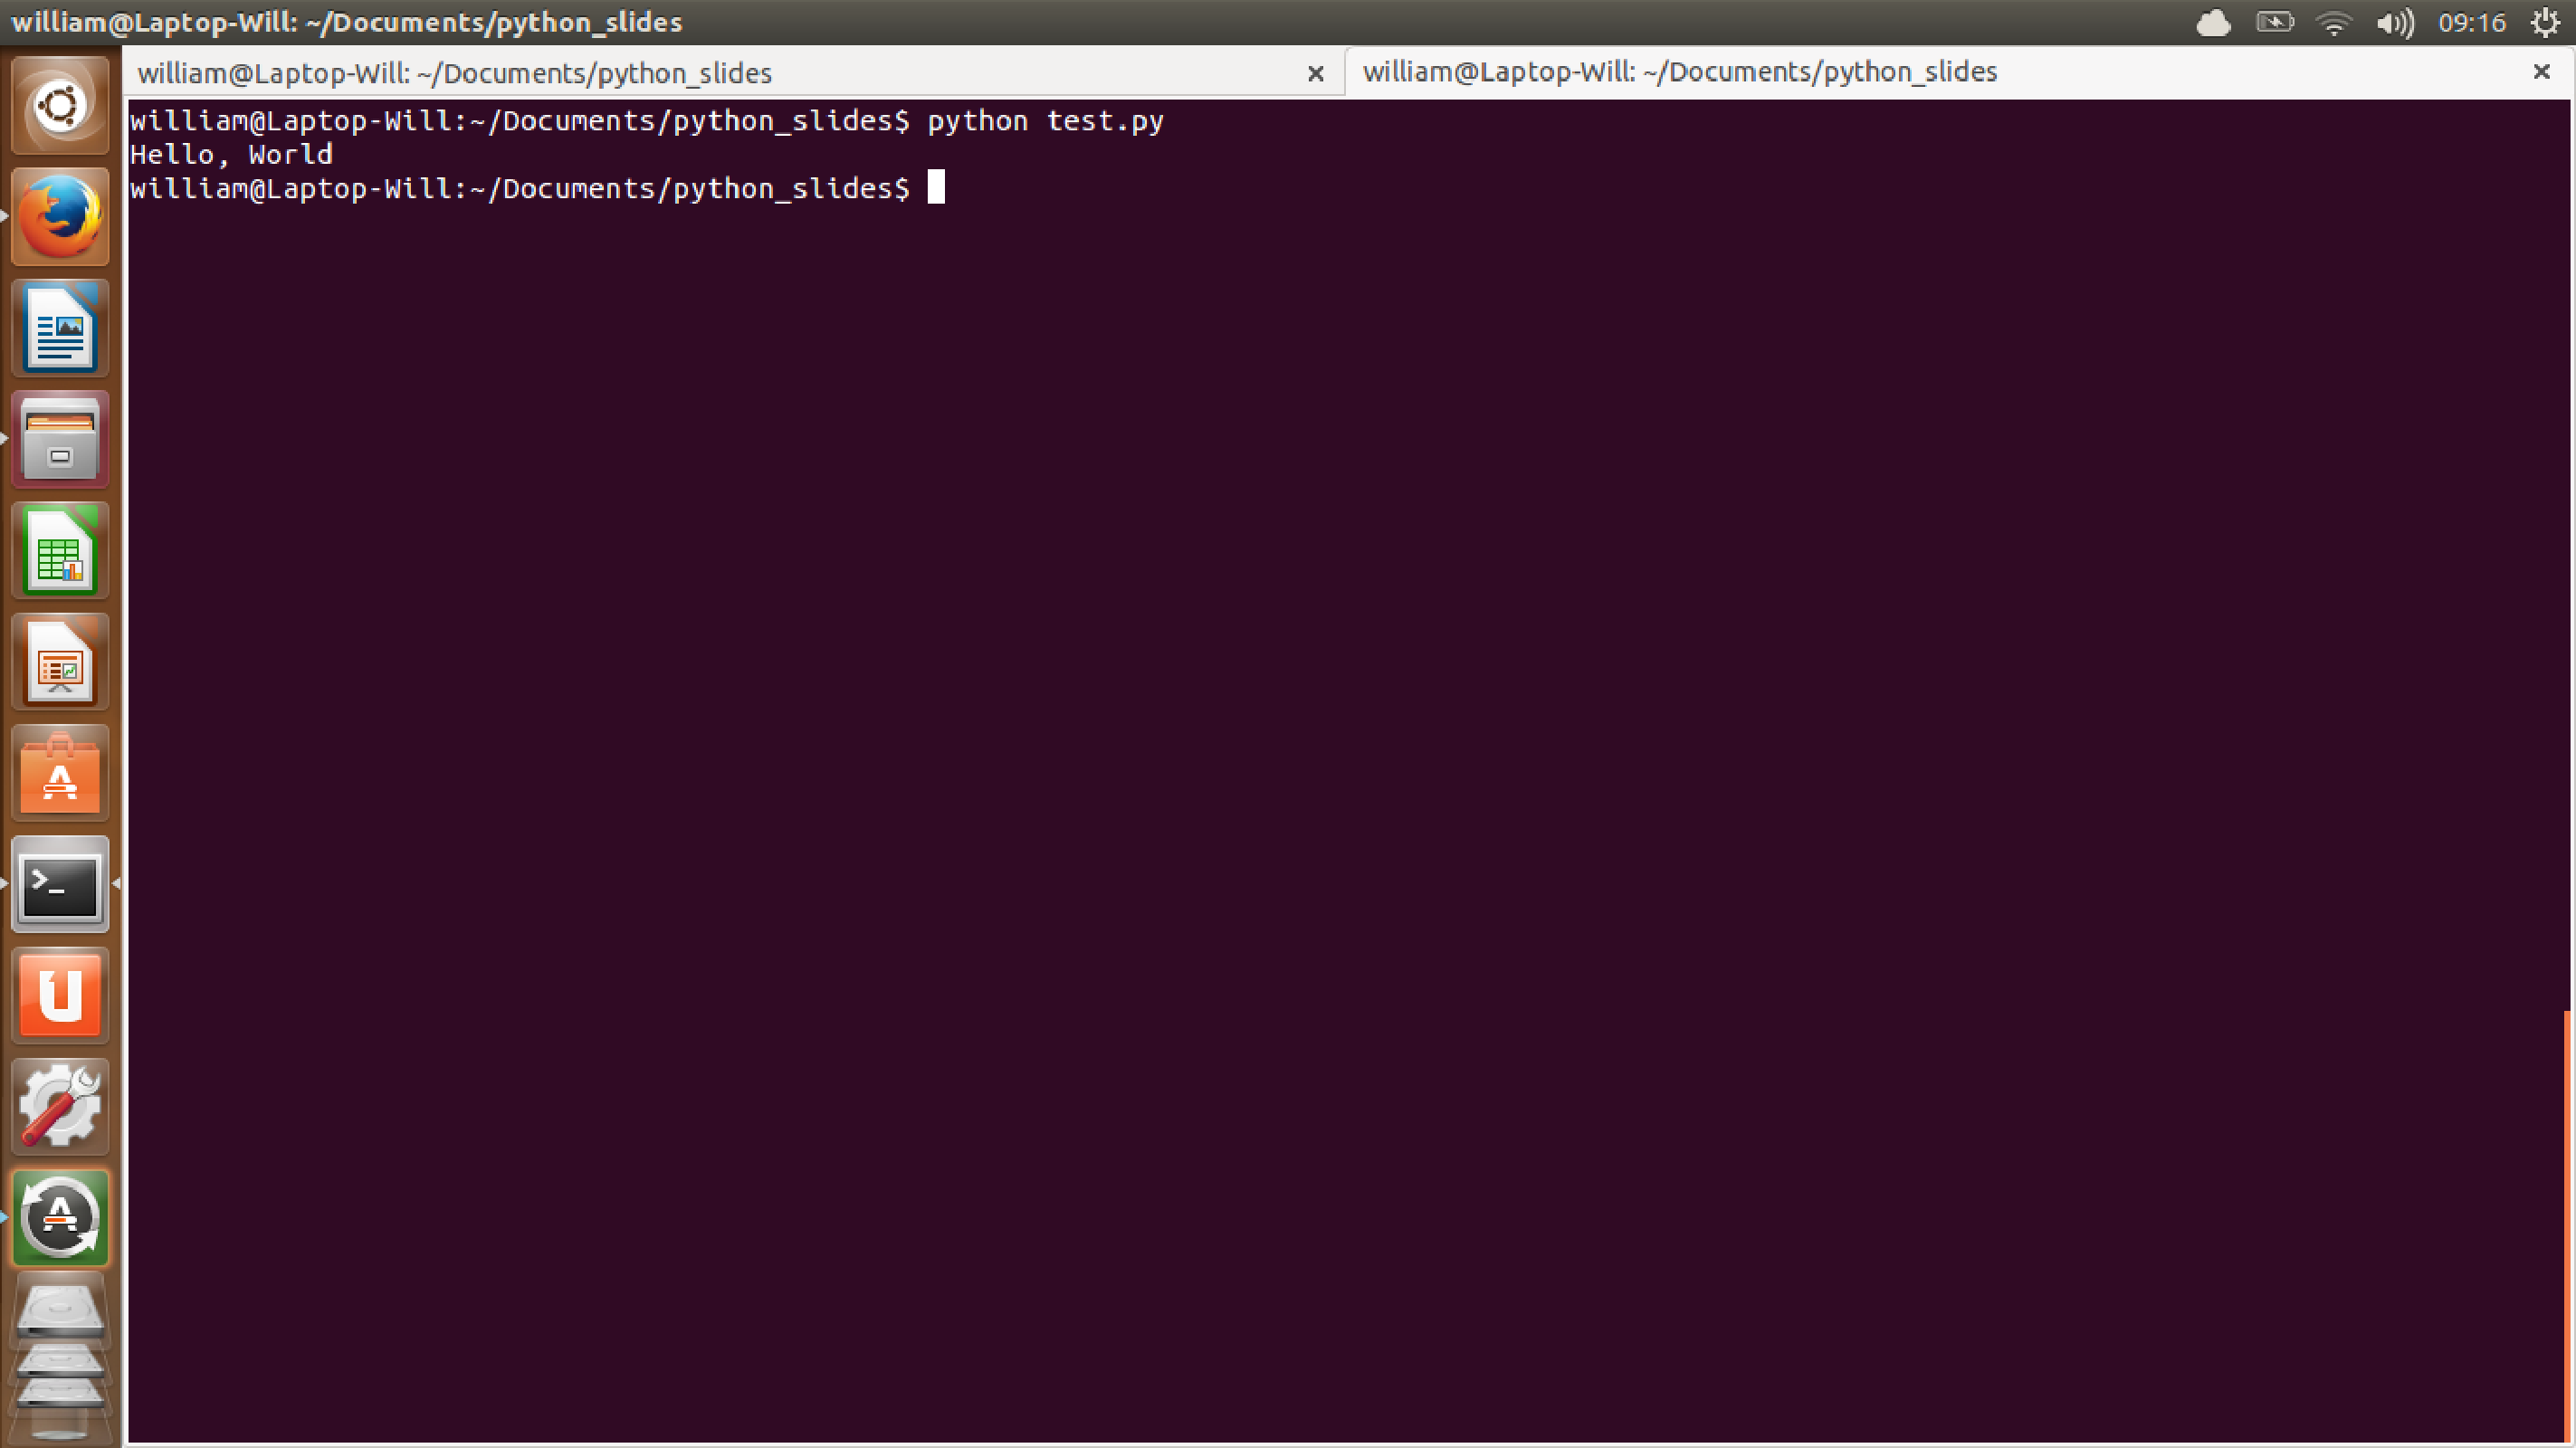
\includegraphics[width=0.5\textwidth]{term.pdf}
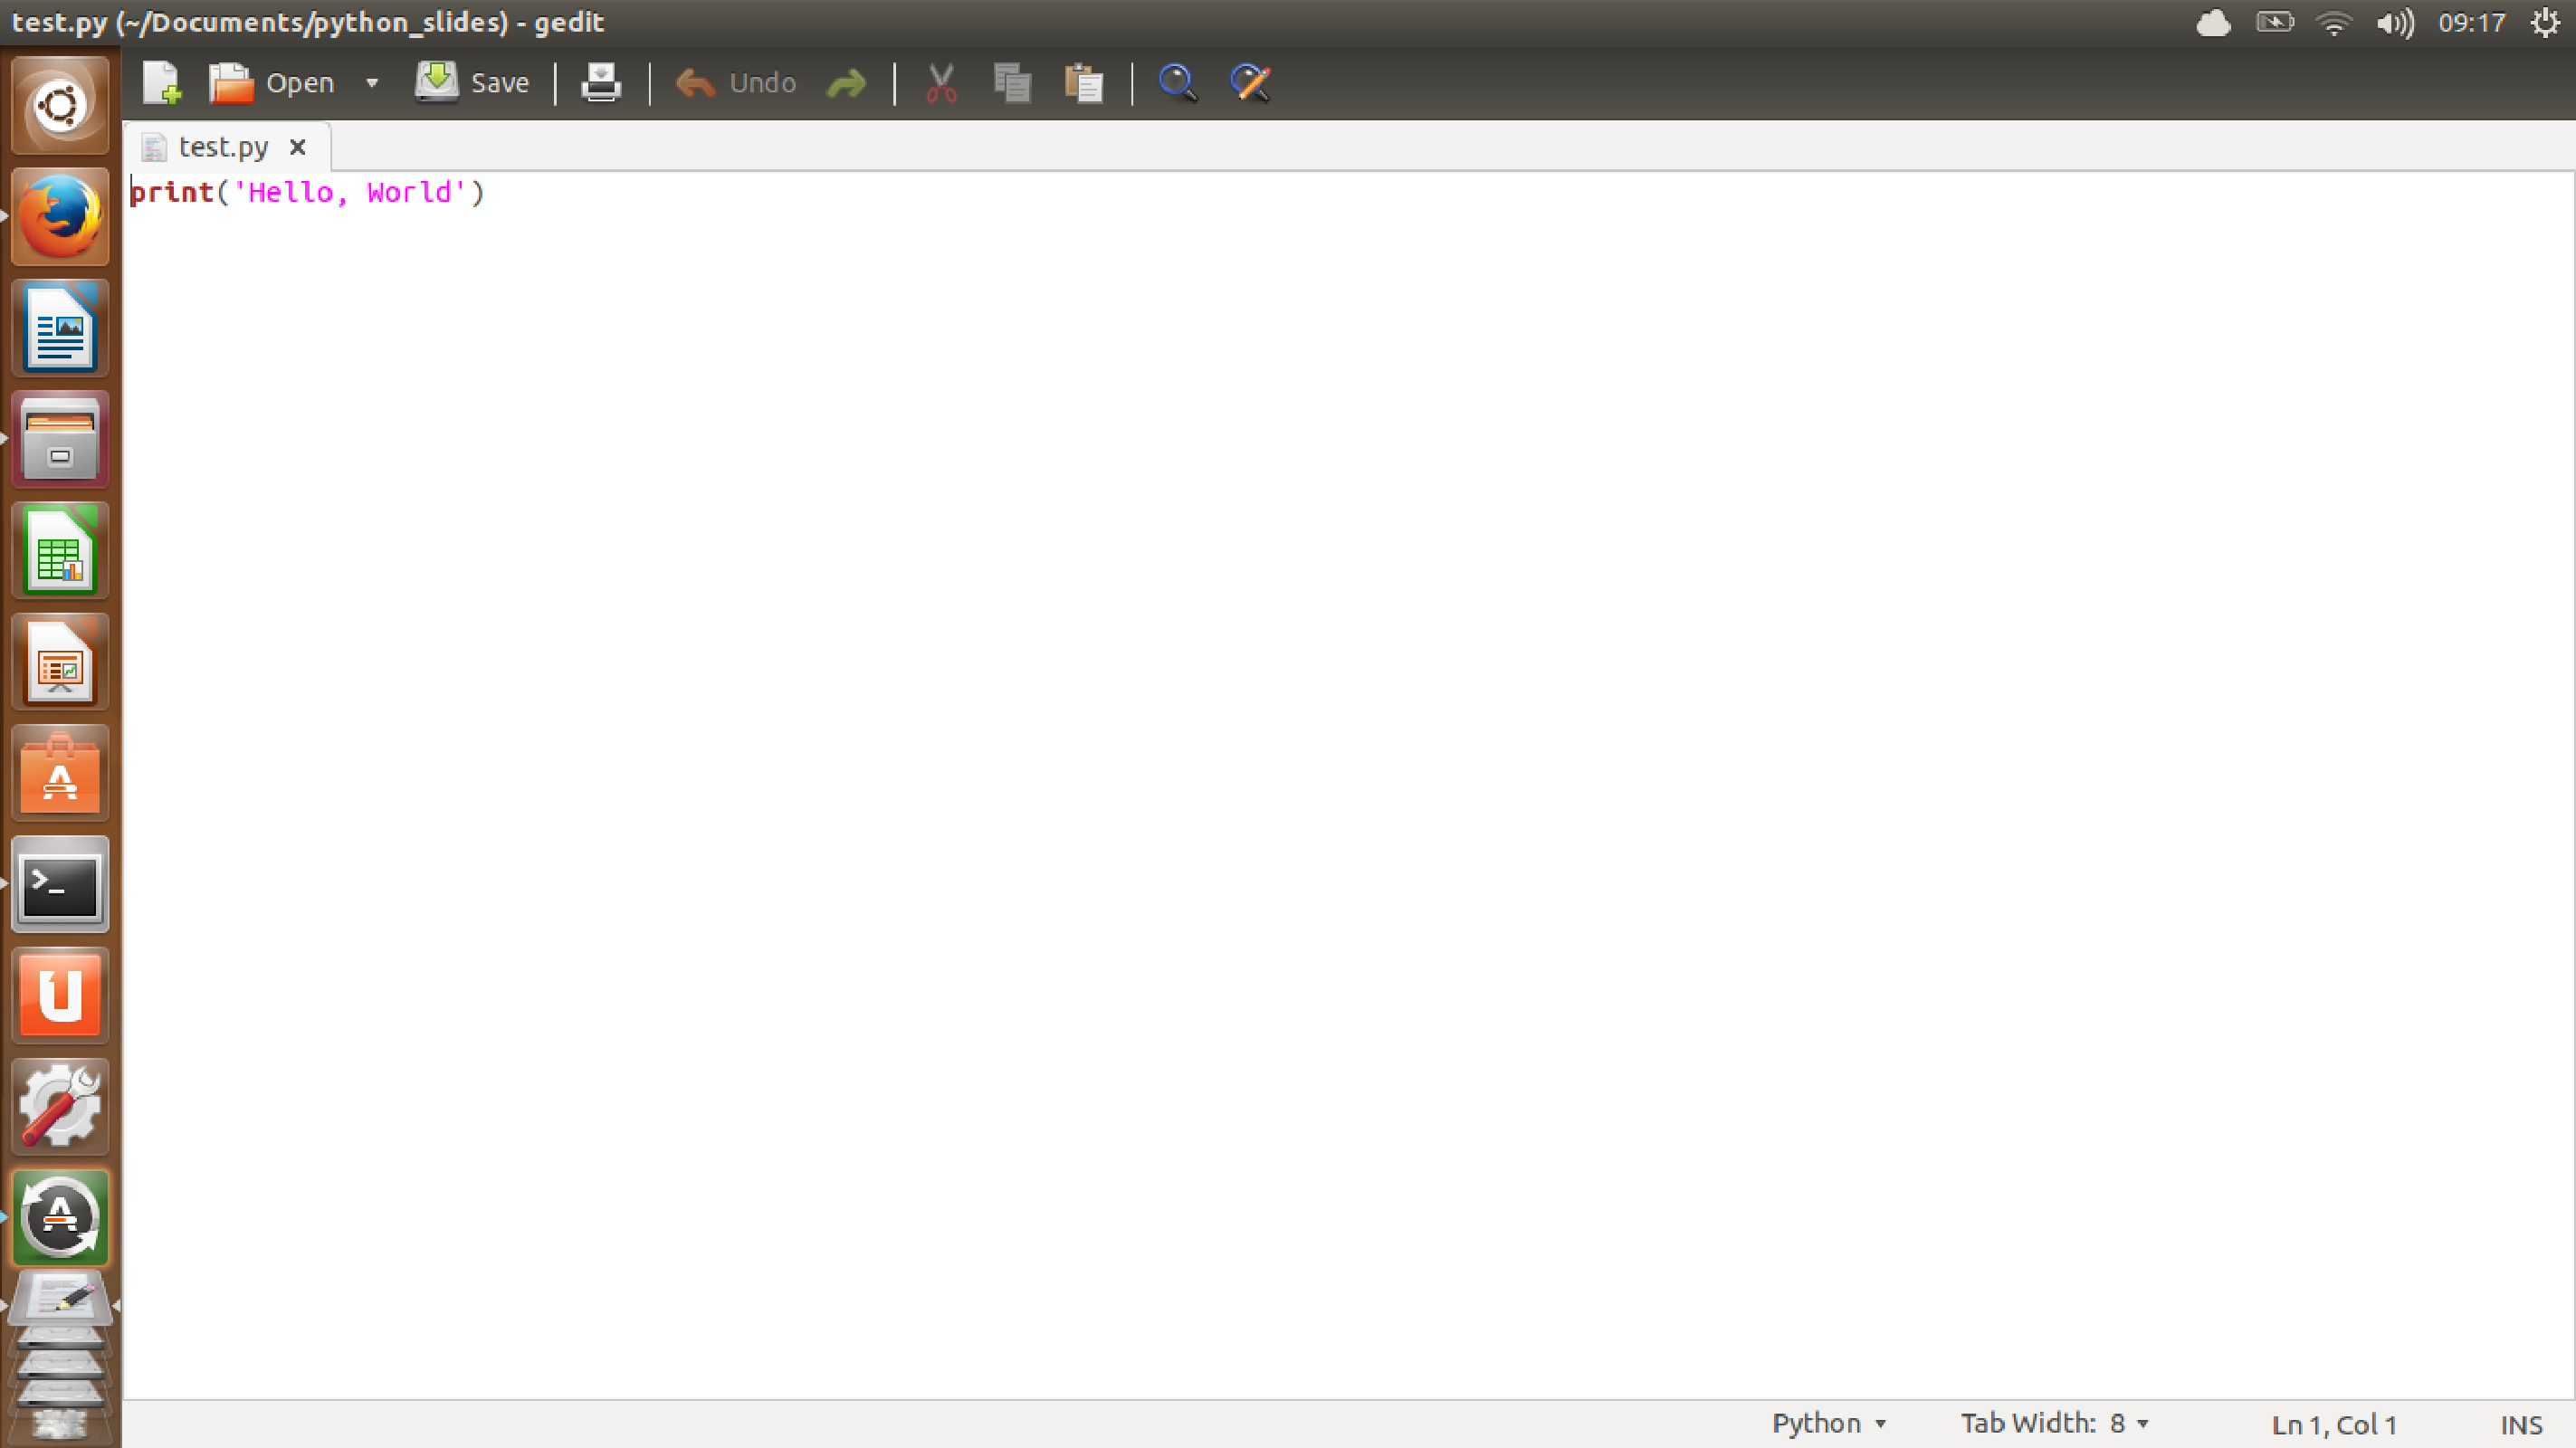
\includegraphics[width=0.5\textwidth]{file.pdf}
\end{exampleblock}
\begin{itemize}
\item Useful for scripts and finished programs.
\end{itemize}
}
\frame{
	\frametitle{Using the IPython Interactive environment}

\begin{itemize}
\item To launch from the command line: ipython
\item Interactive session consists of a number of cells which are ran consecutively.
\end{itemize}
\begin{exampleblock}{}
\centering
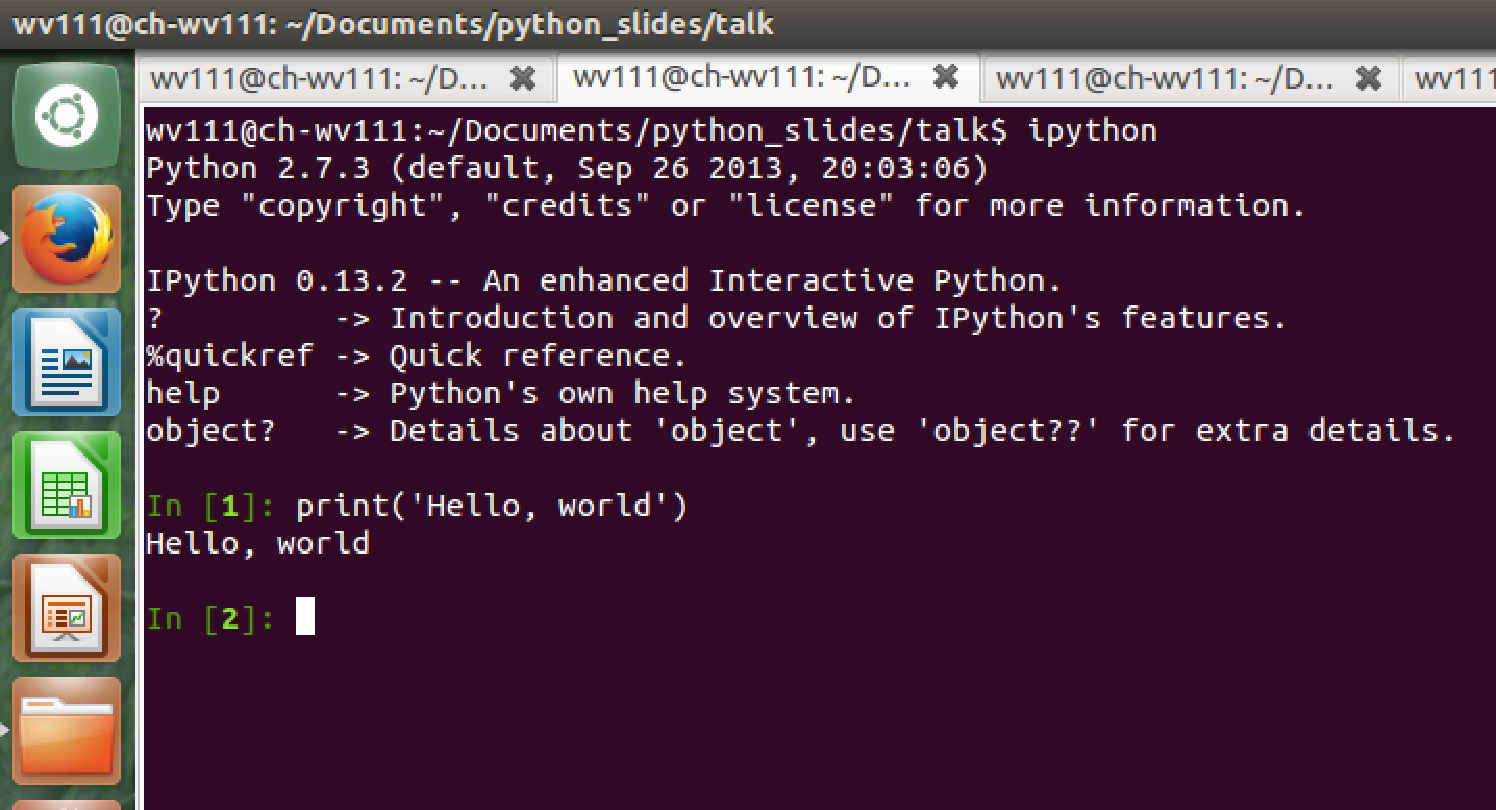
\includegraphics[width=0.5\textwidth]{ipython.pdf}
\end{exampleblock}

\begin{itemize}
\item Useful for quickly testing out simple ideas which can be put into a .py file later.
\item Unfortunately once IPython is closed the code is lost.
\end{itemize}
}
\frame{
	\frametitle{Using the IPython Interactive Notebook}

\begin{itemize}
\item To launch from the command line: ipython notebook --pylab=inline
\item Interactive session consists of a number of cells which can be run in any order.
\item Can insert plain text and latex notes, links to web pages, images and videos.
\end{itemize}
\begin{exampleblock}{}
\centering
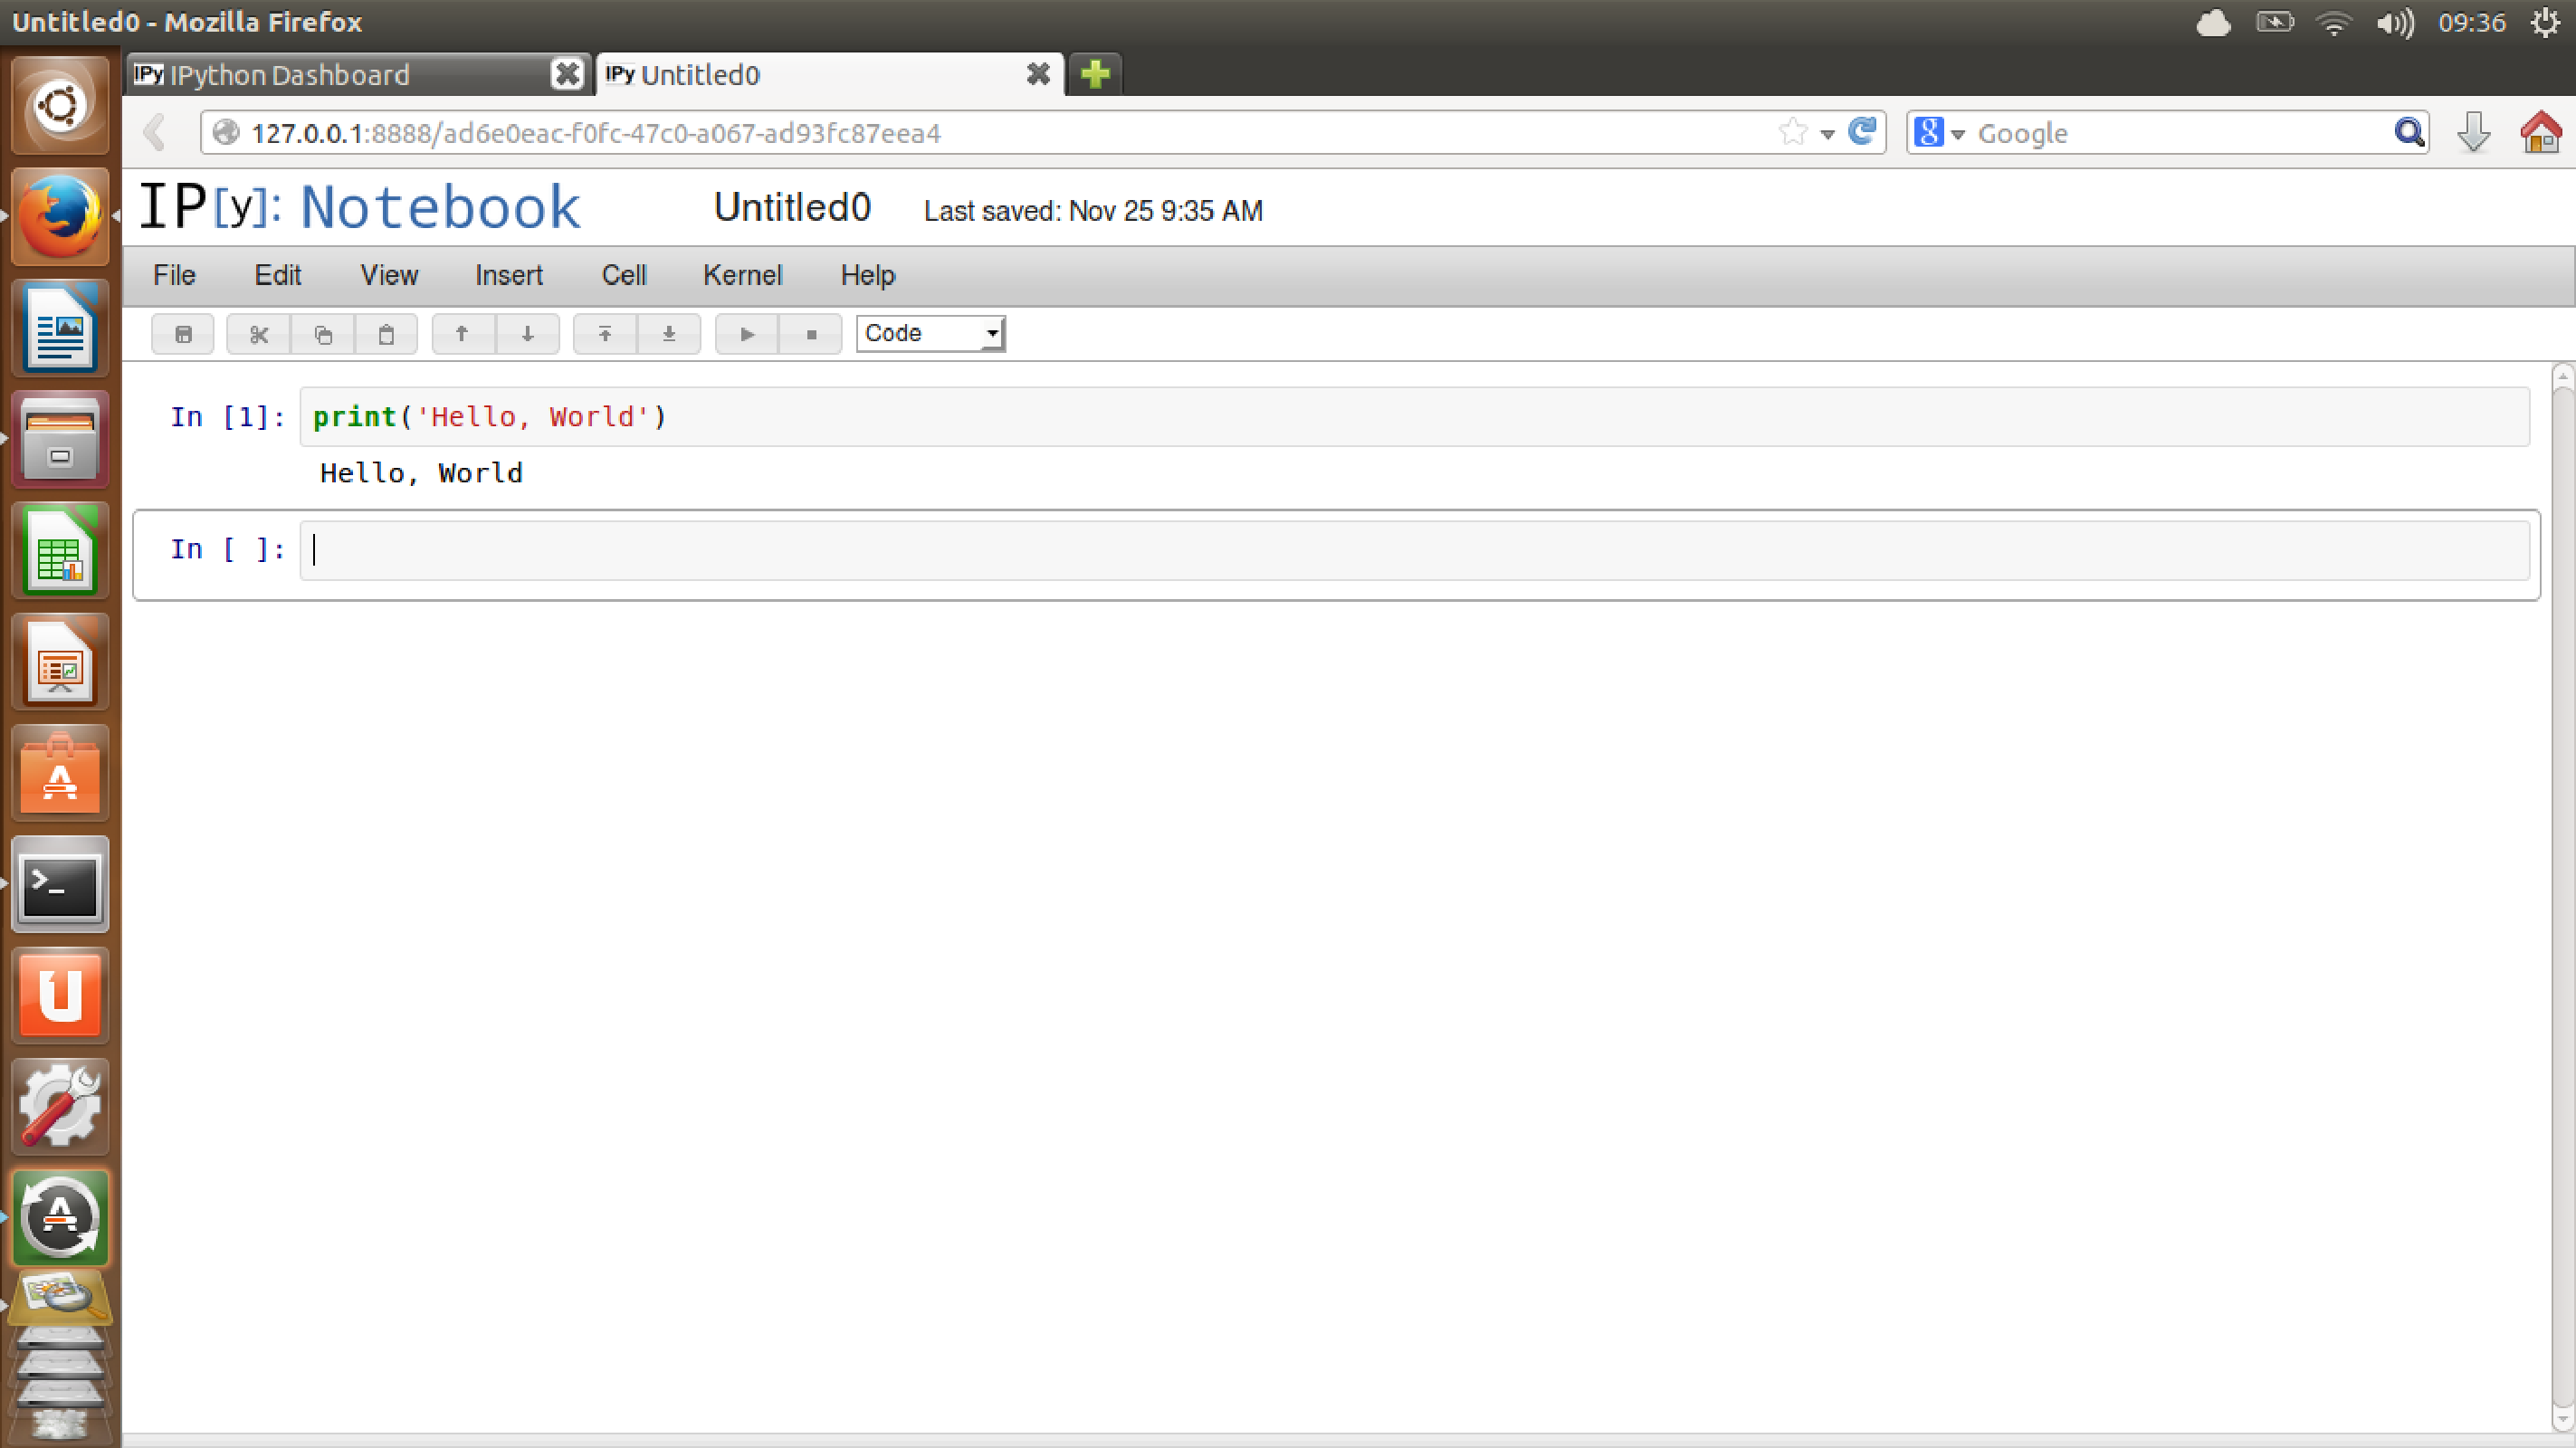
\includegraphics[width=0.5\textwidth]{ipython-notebook.pdf}
\end{exampleblock}
}
\frame{
	\frametitle{Using the IPython Interactive Notebook}
\begin{itemize}
\item Can be used to make a Lab Notebook to analyse data.
\item Graphs generated from the code can be directly placed into the notebook.
\begin{exampleblock}{}
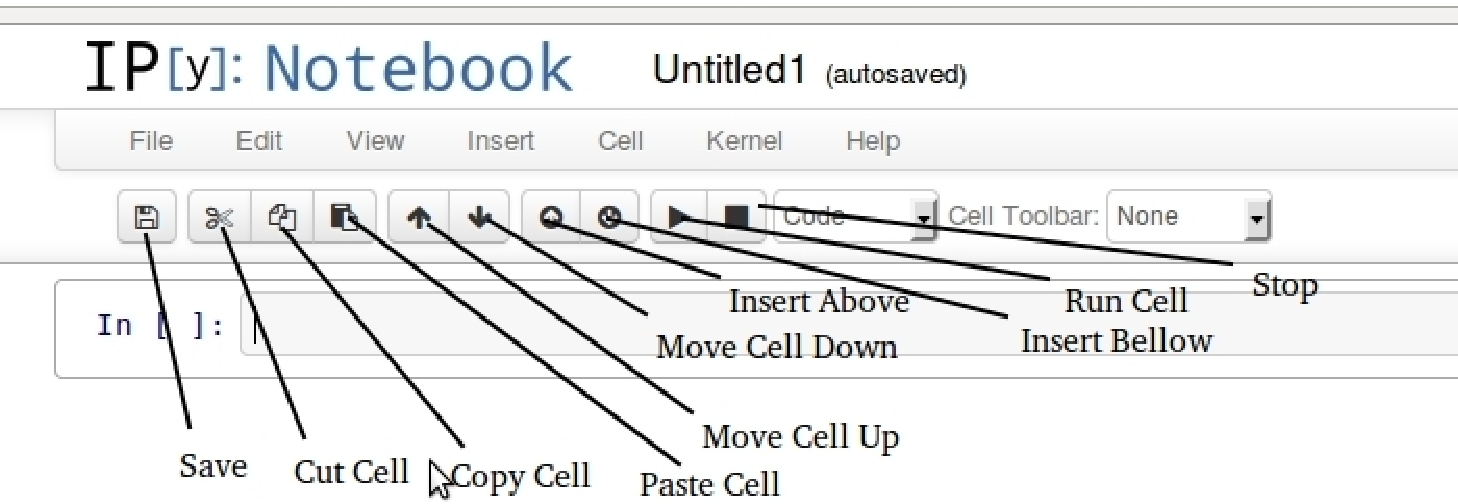
\includegraphics[width=1\textwidth]{dash.pdf}
\end{exampleblock}

\end{itemize}
}

\frame{
	\frametitle{Using the IPython Interactive Notebook}

\begin{itemize}
\item The order you run the cells in does matter.
\item If in doubt restart the notebook and run again from top to bottom (quickly fix non-obvious problems). 
\end{itemize}
\begin{exampleblock}{}
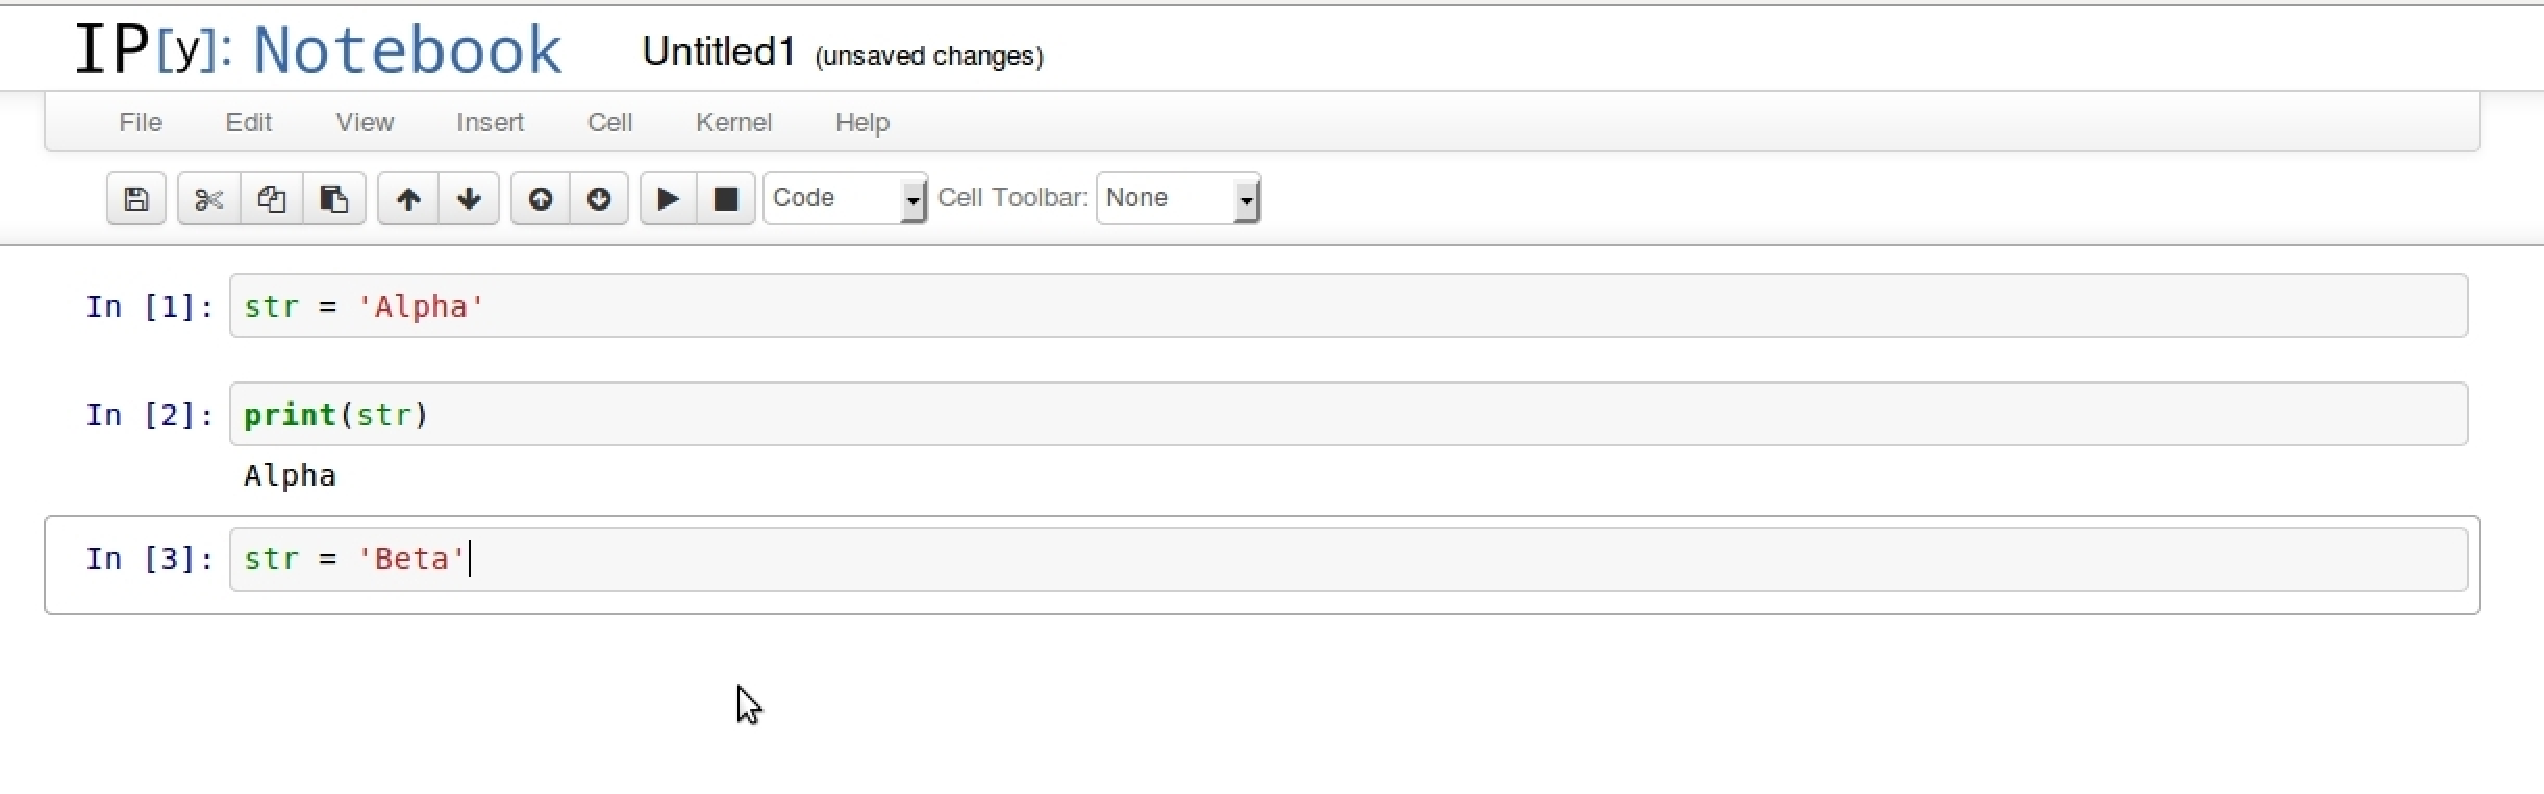
\includegraphics[width=1\textwidth]{order-1.pdf}
\\
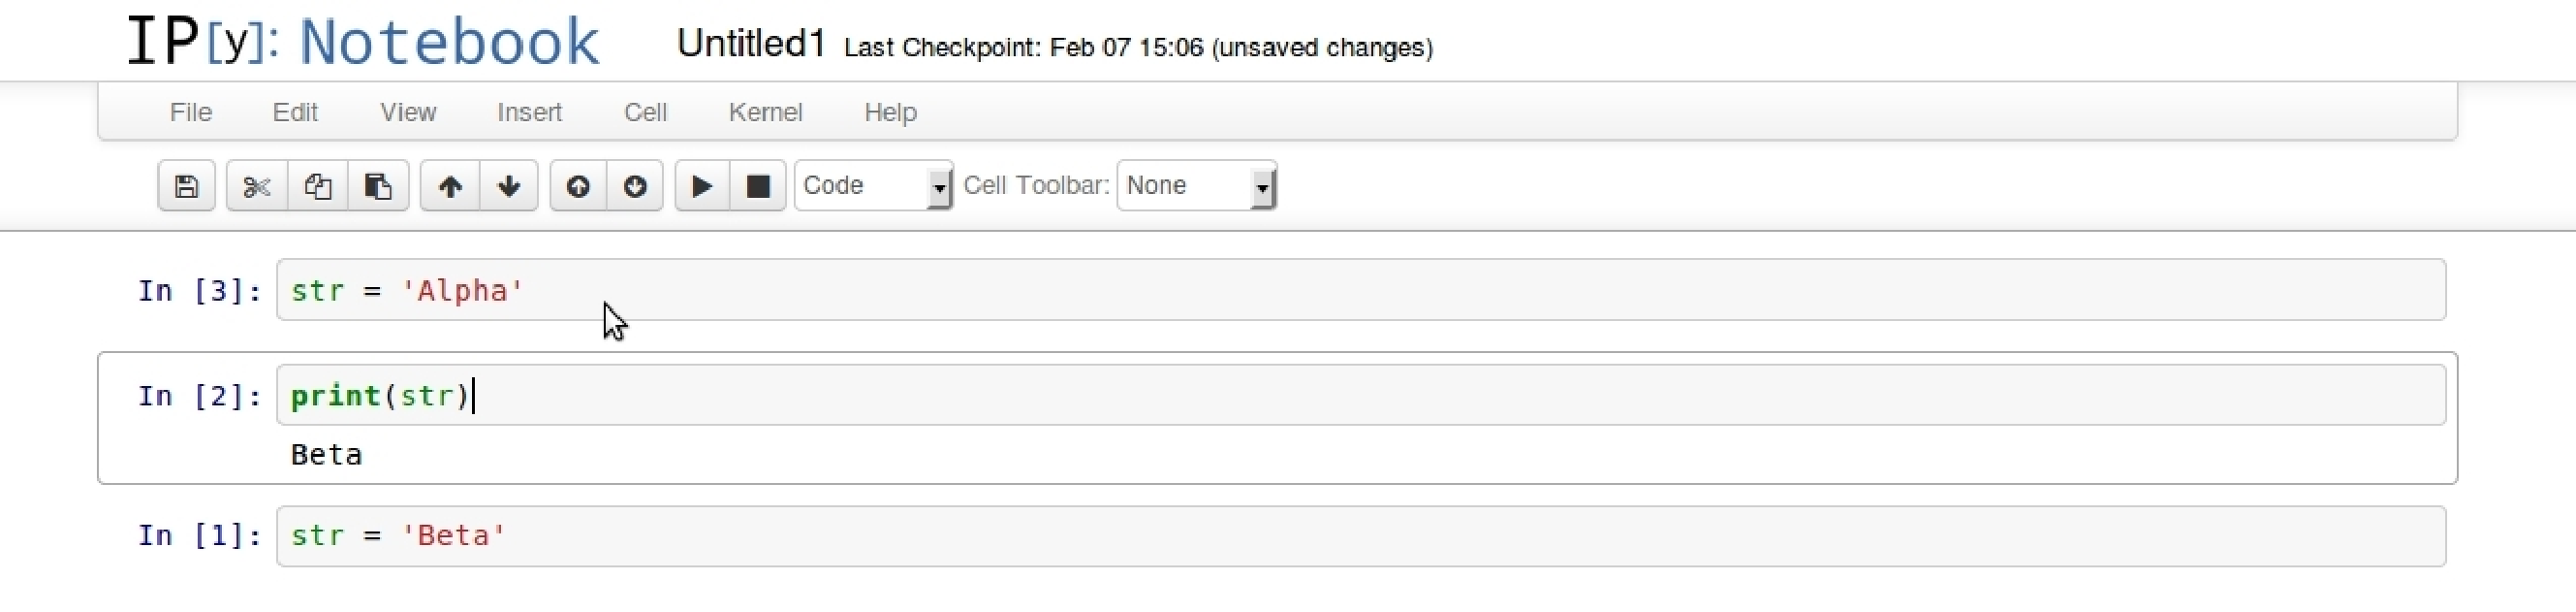
\includegraphics[width=1\textwidth]{order-2.pdf}
\end{exampleblock}

}

\frame{
	\frametitle{Other Resources}

\begin{itemize}
\item General python: \href{http://doc.python.org/2/}{http://doc.python.org/2/}
\item Scipy: \href{www.scipy.org}{www.scipy.org}
\item Numpy: \href{www.numpy.org}{www.numpy.org}
\item Further tutorials: 
\item Anaconda distribution: \href{https://store.continuum.io/cshop/anaconda/}{https://store.continuum.io/cshop/anaconda/}
\end{itemize}
}

\frame{
	\frametitle{Tips}
\begin{itemize}
\item Write code which is easy to read. (Code should be written for Humans not computers)
\item The simplest solution to a problem is almost always the best.
\item Ask questions. It is easy to have misconceptions about programming.
\end{itemize}
}
\end{document}
